\documentclass[11pt]{article}
\usepackage[a4paper,top=23mm,bottom=25mm,left=24mm,right=24mm]{geometry}
\usepackage{fontspec}
\usepackage{unicode-math}
\setmainfont{texgyretermes-regular.otf}[
  BoldFont=texgyretermes-bold.otf,
  ItalicFont=texgyretermes-italic.otf,
  BoldItalicFont=texgyretermes-bolditalic.otf]
\setsansfont{texgyreheros-regular.otf}[BoldFont=texgyreheros-bold.otf]
\setmonofont{lmmono10-regular.otf}[Scale=MatchLowercase]
\setmathfont{latinmodern-math.otf}
\setmathfont{latinmodern-math.otf}[version=bold,FakeBold=1.5]
\usepackage{microtype}
\usepackage{amsmath}
\usepackage{graphicx}
\usepackage{booktabs}
\usepackage{array}
\usepackage{adjustbox}
\usepackage{pdflscape}
\usepackage{xcolor}
\usepackage{cite}
\usepackage[hidelinks]{hyperref}
\usepackage{caption}
\captionsetup{font=small,labelfont=bf,labelsep=period,justification=justified,singlelinecheck=false}
\setlength{\parindent}{1.4em}
\setlength{\parskip}{0.22em}
\setlength{\emergencystretch}{2em}
\hbadness=2000
\renewcommand{\familydefault}{\rmdefault}
\renewcommand{\baselinestretch}{1.08}


\title{Probabilistic graph completion of historical Chinese incense formulas under source shift}

\author{Author name\\Affiliation, city, country\\Corresponding email}

\date{}

\begin{document}

\maketitle

\begin{abstract}

Historical incense books preserve formulas unevenly, while modern odor datasets describe molecules and rarely recipes. We formulate missing-ingredient recovery as source-shifted probabilistic set completion. Xiangji-CGIR combines a directed material graph with a Laplace-approximated inclusion model and explicit ingredient-count and composition uncertainty. We curated 91 family-unique Chinese incense formulas from six work groups. At 50\% observed context, the graph reached source-macro hidden-component F1 0.365 versus 0.339 for frequency, 0.343 for formula k-nearest neighbours and 0.334 for PureSVD. Removing nine cross-work high-similarity formulas retained the graph advantage, 0.348 versus 0.322. Development-calibrated count intervals achieved 0.825 coverage at nominal 0.80. The full decoder reached F1 0.366, and confirmation on a quarantined work reached 0.577. An 18-material chemical kernel did not improve completion. Co-formulation structure transfers across texts; molecular similarity alone does not represent historical ingredient complementarity.

\end{abstract}

\section{Introduction}

Smell can carry cultural meaning, but it leaves a fragmented archive. Heritage frameworks now treat historic odors as objects that can be identified, described and preserved \cite{ref1}. The Odeuropa data model connects odor sources, emissions, experiences, places and historical language \cite{ref2}. Analytical heritage science has also reconstructed the present smell of a surviving perfume residue by combining gas chromatography, olfactory detection and sensory validation \cite{ref3}. Historical incense formulas pose a different computational problem. The material may no longer survive, and the books may preserve only a name, partial recipe, attributed source or literary description, with no measurable headspace sample.

Computational olfaction has learned useful mappings from molecular structure or mass spectra to perceptual descriptors \cite{ref4,ref5,ref6,ref7,ref8}. Mixture models now predict descriptors for pairs of aroma chemicals \cite{ref9}, and inverse design can optimize modern essential-oil mixtures against a requested scent profile \cite{ref10}. These systems start from molecules, spectra or controlled vocabulary. They do not recover a historical natural-material formula from incomplete evidence transmitted through different texts. Historical language processing addresses orthographic variation and sparse annotation \cite{ref11}, while recipe information extraction resolves ingredients and quantities from modern text \cite{ref12}. Neither line of work supplies a source-shifted benchmark for historical formula completion. Nearest-neighbour retrieval and low-rank recommendation test whether a historical graph adds information beyond local formula analogy or latent co-occurrence \cite{ref16,ref17}. Development-held-out interval expansion tests whether its count uncertainty transfers \cite{ref18}.

We define a formula as a sparse set of aromatic materials with relative dry-mass ratios. Given its title, source identifier and a known subset of ingredients, the task is to recover the hidden materials and their proportions. This setting tests a practical scholarly operation: completing a damaged or selectively transmitted formula from patterns learned in other works. It also exposes the central statistical difficulty. Incense vocabularies are long-tailed, formula sizes vary, and source traditions differ. A random record split would let near-identical textual and material conventions leak across training and test sets.

Xiangji-CGIR makes four contributions. First, it introduces a provenance-rich reference set of 91 family-unique formulas from six Chinese incense work groups, with stable source locators, canonical material identifiers and source-blocked splits. Second, it represents each formula as a hyperedge and converts training-only co-occurrence counts into a directed posterior-predictive material graph. Third, it couples that graph to a Laplace-approximated generalized Bayesian inclusion decoder, an empirical-Bayes ingredient-count distribution and a residual-scaled Dirichlet composition distribution. Fourth, it measures the contribution of chemistry through development ablations, an auxiliary inverse-odor task and shuffled material-chemistry assignments. Co-formulation structure transfers across historical works; title and source channels add no reliable gain beyond the graph, and pairwise chemical similarity does not improve completion.

\section{Related Work}

This study joins three research lines that are usually evaluated separately. Computational olfaction predicts perceptual descriptors from molecular structure, spectra or controlled mixtures \cite{ref4,ref5,ref6,ref7,ref8,ref9,ref10}. Historical-language and recipe-processing systems recover entities and quantities from text \cite{ref11,ref12}. Multi-label learning and recommender systems recover missing labels from sparse co-occurrence structure \cite{ref13,ref16,ref17}. Xiangji-CGIR uses chemical representations as an auditable evidence layer, but its primary output is a structured completion of natural-material formulas rather than a molecular odor prediction.

The closest statistical formulation is multi-label set completion under domain shift. Sparse Bayesian multi-label models use label correlations to regularize prediction \cite{ref13}, while WILDS formalizes evaluation when deployment domains differ from training environments \cite{ref14}. Historical formula books create both problems at once: ingredients are correlated within a formula, and each work carries its own vocabulary, editing history and compositional conventions. We therefore treat each work as a domain and rebuild every prevalence, graph and text statistic inside the training fold.

Our uncertainty design also draws on two distinct traditions. The inclusion decoder uses a Laplace approximation around a regularized, class-weighted logistic optimum, whereas the total-count interval is recalibrated from work-held-out residuals using split-conformal logic \cite{ref18}. Composition is evaluated in simplex geometry \cite{ref19}. These components answer different questions—whether a material is present, how many materials remain, and how mass is distributed—and are assessed separately rather than collapsed into one confidence score.

\section{Problem Formulation and Dataset}

\subsection{Corpus Construction and Provenance}

We extracted formula candidates from public-domain Chinese incense texts and their Wikisource transcriptions. Each candidate stored the work and edition identifier, formula title, verbatim source span, stable revision URL, line locator, transcription hash, material mentions, quantity strings, process mentions and rights statement. The curation protocol separated aromatic materials from binders, liquids and processing aids. It converted historical mass expressions to qian on a relative basis, summed repeated mentions and normalized aromatic mass to one. Records with an unresolved aromatic quantity, list boundary or formula identity were excluded without imputation.

Canonicalization mapped material mentions to an ontology identifier while retaining the surface form and identity status. Grade terms for agarwood remained separate identifiers. Four contextually resolved characters carry explicit resolution records. Candidate families were compared by normalized title, material-set overlap, ratio pattern and source genealogy. One checked representative was retained per provisional family. The resulting version 0.1 reference set contains 91 formulas; 29 screened candidates were excluded. All transformations are executable and hash checked.

\subsection{Prediction Task and Observation Mechanism}

For formula \(i\), let \(q_{ij}\) be the converted aromatic mass of material \(j\), \(S_i\) its material support and \(M\) the training vocabulary size. Aromatic masses were closed to the simplex as

\begin{equation}
\label{eq:composition-closure}
\mathbf{w}_i\in\Delta^{M-1},\qquad w_{ij}=\frac{q_{ij}}{\sum_{k\in S_i}q_{ik}},\qquad S_i=\{j:w_{ij}>0\}.
\end{equation}

The model receives title \(t_i\), work identifier \(d_i\) and an observed subset \(O_i\subset S_i\) with the original entries \(\{w_{ij}:j\in O_i\}\). It predicts the hidden set \(H_i=S_i\mathbin{\backslash} O_i\), a complete material set \(\widehat S_i\) and a composition \(\widehat{\mathbf w}_i\).

We generated \(O_i\) deterministically from a cryptographic hash of formula identifier, observation fraction and seed. For \(K_i=|S_i|\), the retained count was

\begin{equation}
\label{eq:mask-cardinality}
r(K_i,f)=\min\{K_i-1,\max[1,\operatorname{round}(fK_i)]\},\qquad |O_i|=r(K_i,f).
\end{equation}

Here \(f\in\{0.25,0.50,0.75\}\). This rule guarantees at least one observed and one hidden in-vocabulary material. The registered primary fraction was 0.50. Five seeds, 17, 29, 43, 71 and 101, changed the observed subset but not the source splits.

\subsection{Source-Blocked Splits}

The Hong work group and its six formulas were removed before vocabulary construction, prior estimation, feature scaling or model selection. Development used five leave-one-work-out folds. Primary evaluation used all ten unordered pairs of the five remaining work groups as test domains, with the other three groups as training data. Family identifiers were disjoint because the reference set contains one representative per checked family. Each test formula appears in four source-pair folds and five mask seeds. We first averaged repeated predictions for a formula, then averaged formulas within a work group, then averaged the five work groups. The historical work is the unit of primary inference.

\begin{table}[htbp]
\centering
\small
\caption{Notation used in the mathematical formulation.}
\label{tab:1}
\begin{adjustbox}{max width=\linewidth}
\begin{tabular}{@{}ll@{}}
\toprule
\textbf{Symbol} & \textbf{Meaning} \\
\midrule
i, j, d & Formula, material and historical-work indices \\
S\_i, O\_i, H\_i & Complete, observed and hidden material sets for formula i \\
q\_ij, w\_ij & Converted aromatic mass and closed mass fraction \\
pi\_j, pi\_j|d & Global and source-conditioned material prevalence \\
G\_ab & Directed posterior-predictive affinity from material a to b \\
g\_ij, u\_ij & Source-deviation feature and observed-material indicator \\
phi\_ij, x\_ij, z\_ij & Core, complete and standardized candidate-feature vectors \\
theta, Sigma & Inclusion coefficients and Laplace covariance \\
p\_ij & Posterior-approximated inclusion probability \\
K\_i, K-hat\_i & True and predicted total ingredient count \\
mu\_ij, W\_i & Predicted mean composition and composition random vector \\
L\_tr, L\_r, B & Candidate rows, positive ratio rows and chemical-profile bins \\
D, I\_d, A\_i & Number of works, formulas in work d and repeated evaluations of formula i \\
\bottomrule
\end{tabular}
\end{adjustbox}
\end{table}

\section{Xiangji-CGIR Method}

\subsection{Model Overview}

Xiangji-CGIR separates formula completion into candidate inclusion, total ingredient count and composition. Figure 1 summarizes the training-only information flow and the source-blocked evaluation design.

\begin{figure}[htbp]
\centering
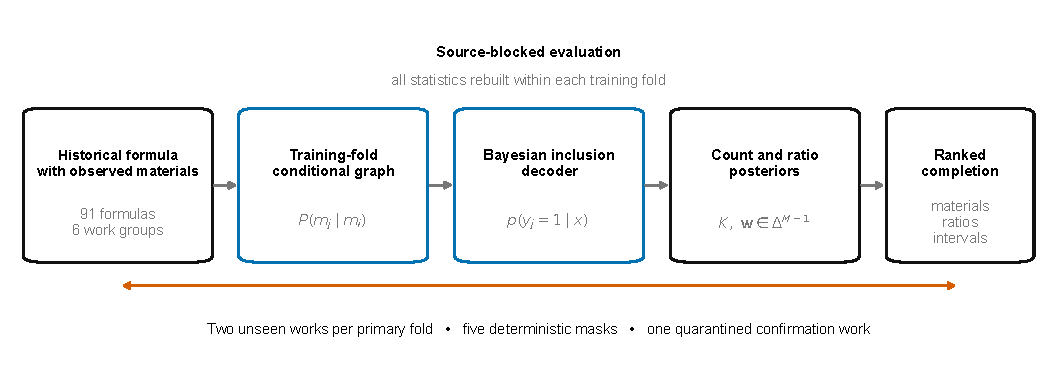
\includegraphics[width=0.98\linewidth]{figures/fig1_workflow.pdf}
\caption{Xiangji-CGIR workflow and evaluation design. Historical formulas supply titles, source identifiers and deterministically observed material subsets. A training-fold directed material graph generates candidate affinities. A Laplace-approximated generalized Bayesian logistic decoder produces inclusion probabilities, after which count and composition uncertainty models define a ranked completion with intervals. Every statistic is rebuilt within the training fold. The primary design holds out two entire work groups per fold and uses five deterministic masks; the Hong work is reserved for confirmation.}
\label{fig:1}
\end{figure}

\subsection{Directed Posterior-Predictive Material Graph}

Each training formula defines a hyperedge over its aromatic materials. Among \(N\) training formulas, let \(c_a\) count formulas containing material \(a\), \(c_{ab}\) count formulas containing both \(a\) and \(b\), and \(c_{dj}\) count material \(j\) in the \(N_d\) formulas from work \(d\). Global and work-specific prevalence estimates were

\begin{equation}
\label{eq:prevalence-priors}
\pi_j=\frac{c_j+1/2}{N+1},\qquad \pi_{j\mid d}=\frac{c_{dj}+\lambda_s\pi_j}{N_d+\lambda_s},\qquad \lambda_s=5.
\end{equation}

The directed posterior-predictive co-formulation edge was

\begin{equation}
\label{eq:directed-graph}
G_{ab}=\frac{c_{ab}+\alpha\pi_b}{c_a+\alpha},\qquad \alpha=2,\qquad G_{aa}=1.
\end{equation}

For the locked arithmetic-mean reducer, graph affinity for candidate \(j\) was

\begin{equation}
\label{eq:graph-affinity}
a^{(G)}_{ij}=\frac{1}{|O_i|}\sum_{a\in O_i}G_{aj}.
\end{equation}

Direction matters because \(G_{ab}\) generally differs from \(G_{ba}\). During training, prevalence estimates and the graph for formula \(i\) were rebuilt without that formula, preventing its target labels from contributing to its own features.

\subsection{Generalized Bayesian Inclusion Decoder}

The title encoder mapped each title to an L2-normalized character 1- and 2-gram TF-IDF vector \(\mathbf v(t)\). For candidate \(j\), the normalized training-title centroid and its similarity to formula \(i\) were

\begin{equation}
\label{eq:title-affinity}
\mathbf u_j=\frac{\sum_{r=1}^{N}y_{rj}\mathbf v(t_r)}{\left\|\sum_{r=1}^{N}y_{rj}\mathbf v(t_r)\right\|_2},\qquad a^{(T)}_{ij}=\mathbf v(t_i)^{\top}\mathbf u_j.
\end{equation}

The active candidate feature vector in the locked decoder was

\begin{equation}
\label{eq:candidate-features}
g_{ij}=\operatorname{logit}\pi_{j\mid d_i}-\operatorname{logit}\pi_j,\qquad u_{ij}={\bf1}(j\in O_i),\qquad \mathbf x_{ij}=[\operatorname{logit}\pi_j,g_{ij},a^{(T)}_{ij},a^{(G)}_{ij},u_{ij},u_{ij}\log w_{ij}]^{\top}.
\end{equation}

Training-fold means \(\boldsymbol\mu_x\) and standard deviations \(\mathbf s_x\) supplied elementwise standardization, \(\mathbf z_{ij}=(\mathbf x_{ij}-\boldsymbol\mu_x)\oslash\mathbf s_x\). An odor-similarity slot was present in the software interface but identically zero because the primary formulas contain no independent odor target. Chemistry channels were disabled in the locked model after development selection. For a held-out work, \(\pi_{j\mid d_i}\) defaults to \(\pi_j\), so the source-deviation coordinate is exactly zero rather than using information from the test work.

Let \(n\) index the \(L_{\mathrm{tr}}\) formula-candidate training rows, \(y_n\in\{0,1\}\) indicate material presence, and \(\widetilde{\mathbf z}_n=[1,\mathbf z_n^{\top}]^{\top}\). The conditional inclusion model was

\begin{equation}
\label{eq:logistic-model}
p_n(\boldsymbol\theta)=\sigma(\widetilde{\mathbf z}_n^{\top}\boldsymbol\theta),\qquad \sigma(u)=\frac{1}{1+\exp(-u)}.
\end{equation}

If \(N_1\) and \(N_0\) denote positive and negative candidate rows, class weights were \(\omega_n=N/(2N_1)\) for \(y_n=1\) and \(\omega_n=N/(2N_0)\) otherwise. With intercept precision \(10^{-6}\) and coefficient prior variance \(C=3.0\), the generalized maximum-a-posteriori estimate minimized

\begin{equation}
\label{eq:map-objective}
\mathcal L(\boldsymbol\theta)=\sum_{n=1}^{L_{\mathrm{tr}}}\omega_n[\log(1+\exp\eta_n)-y_n\eta_n]+\frac{1}{2}\boldsymbol\theta^{\top}\boldsymbol\Lambda\boldsymbol\theta,\qquad \widehat{\boldsymbol\theta}=\arg\min_{\boldsymbol\theta}\mathcal L(\boldsymbol\theta),\quad \eta_n=\widetilde{\mathbf z}_n^{\top}\boldsymbol\theta.
\end{equation}

Here \(\boldsymbol\Lambda=\operatorname{diag}(10^{-6},C^{-1},\ldots,C^{-1})\). At \(\widehat{\boldsymbol\theta}\), the Laplace covariance and generalized posterior approximation were

\begin{equation}
\label{eq:laplace-posterior}
\boldsymbol\Sigma=\left[\widetilde{\mathbf Z}^{\top}\operatorname{diag}\{\omega_n\widehat p_n(1-\widehat p_n)\}\widetilde{\mathbf Z}+\boldsymbol\Lambda\right]^{+},\qquad \boldsymbol\theta\mid\mathcal D\approx\mathcal N(\widehat{\boldsymbol\theta},\boldsymbol\Sigma).
\end{equation}

Class balancing changes the effective prior odds. The implementation restores the training-population odds with \(\delta=\log(N_1/N_0)\) and uses the logistic-normal approximation

\begin{equation}
\label{eq:predictive-probability}
v_{ij}=\widetilde{\mathbf z}_{ij}^{\top}\boldsymbol\Sigma\widetilde{\mathbf z}_{ij},\qquad \widehat p_{ij}=\sigma\left(\frac{\widetilde{\mathbf z}_{ij}^{\top}\widehat{\boldsymbol\theta}+\delta}{\sqrt{1+\pi v_{ij}/8}}\right).
\end{equation}

Central 80\% parameter-induced probability intervals came from \(B\) draws \(\boldsymbol\theta^{(b)}\sim\mathcal N(\widehat{\boldsymbol\theta},\boldsymbol\Sigma)\) and \(p_{ij}^{(b)}=\sigma(\widetilde{\mathbf z}_{ij}^{\top}\boldsymbol\theta^{(b)}+\delta)\). These intervals quantify coefficient uncertainty, not future Bernoulli outcomes. A separate 20,000-step Metropolis-Hastings check on a synthetic logistic problem produced mean absolute predictive difference 0.0016 from the Laplace implementation.

All global prevalence, source prevalence, title-centroid and graph features used leave-one-formula-out values for training examples. Observed materials were forced into the output set after prediction.

\subsection{Ingredient Count and Composition Uncertainty}

We modeled ingredient count separately because inclusion probabilities rank materials but do not determine where the ranked list should stop. For support \(k\in\{1,\ldots,K_{\max}\}\), global and work-shrunk count distributions were

\begin{equation}
\label{eq:count-priors}
p_0(k)=\frac{n_k+1/2}{N+K_{\max}/2},\qquad p_d(k)=\frac{n_{dk}+\lambda_k p_0(k)}{N_d+\lambda_k},\qquad \lambda_k=3.
\end{equation}

Given \(o=|O_i|\) and the registered fraction \(f\), the exact deterministic-mask likelihood yields

\begin{equation}
\label{eq:count-posterior}
p(K_i=k\mid d_i,o,f)\propto p_{d_i}(k){\bf1}\{k\ge\max(1,o)\}{\bf1}\{r(k,f)=o\}.
\end{equation}

For an unseen work, \(p_{d_i}\) defaults to \(p_0\). The selected formula size was the posterior median

\begin{equation}
\label{eq:count-decision}
\widehat K_i=\min\left\{k:\sum_{h=1}^{k}p(K_i=h\mid d_i,o,f)\ge\frac{1}{2}\right\},
\end{equation}

which is the Bayes action under absolute count loss. The top \(\widehat K_i\) inclusion probabilities defined \(\widehat S_i\), with observed materials forced into the ranking. This mask-conditioned count posterior is an evaluation model for known \(f\); when the observation process is unknown, the software falls back to the unconditioned work or global count distribution.

For each present training material, ridge regression mapped the standardized candidate features to log composition. With \(L_r\) positive training rows, target \(\ell_n=\log w_n\) and penalty \(\rho=1\), it solved

\begin{equation}
\label{eq:ratio-ridge}
\mathcal R(\mathbf b)=\sum_{n=1}^{L_r}(\ell_n-\widetilde{\mathbf z}_n^{\top}\mathbf b)^2+\rho\|\mathbf b\|_2^2,\qquad \widehat{\mathbf b}=\arg\min_{\mathbf b}\mathcal R(\mathbf b).
\end{equation}

For the selected set \(\widehat S_i\), exponentiation and closure supplied the compositional mean

\begin{equation}
\label{eq:ratio-closure}
r_{ij}=\exp(\widetilde{\mathbf z}_{ij}^{\top}\widehat{\mathbf b}),\qquad \mu_{ij}=\frac{r_{ij}}{\sum_{h\in\widehat S_i}r_{ih}},\quad j\in\widehat S_i.
\end{equation}

If \(s_r^2\) is the mean squared training residual on the log-ratio scale, the implementation sets \(\kappa=\operatorname{clip}(1/\max[s_r^2,0.01],2,100)\) and \(\alpha_{ij}=\max(\kappa\mu_{ij},10^{-3})\), then draws

\begin{equation}
\label{eq:dirichlet-composition}
\mathbf W_{i,\widehat S_i}\sim\operatorname{Dirichlet}(\boldsymbol\alpha_i).
\end{equation}

The 10th and 90th marginal quantiles of 200 draws form central 80\% intervals. This is a residual-scaled uncertainty distribution conditional on the selected set, not a fully Bayesian posterior for set and composition jointly. The registered primary weighted Jaccard used the unconstrained mean \(\boldsymbol\mu_i\). A post-freeze reporting transform holds supplied ratios fixed and allocates the remaining mass over predicted hidden materials:

\begin{equation}
\label{eq:mass-constraint}
\widehat w^{(c)}_{ij}=\begin{cases}w_{ij},&j\in O_i,\\ \left(1-\sum_{a\in O_i}w_{ia}\right)\dfrac{\mu_{ij}}{\sum_{h\in\widehat S_i\mathbin{\backslash} O_i}\mu_{ih}},&j\in\widehat S_i\mathbin{\backslash} O_i,\\0,&\text{otherwise}.\end{cases}
\end{equation}

This transform changes neither material ranking nor selection. It increased post-freeze source-macro weighted Jaccard from 0.387 to 0.427.

The original count interval used the 10th and 90th percentiles of the masked count posterior. We calibrated its width from the five leave-one-work-out development folds \cite{ref18}. For each development prediction, nonconformity was the integer distance from the true count to the original interval, or zero when covered. The finite-sample 80\% quantile over 420 development predictions was one material. We expanded both primary interval endpoints by that value, retaining at least one hidden component. Primary labels did not determine the expansion.

\subsection{Chemoinformatic Evidence Layer}

Targeted searches identified analytical studies for materials in the ontology \cite{ref22,ref23,ref24,ref25,ref26,ref27,ref28,ref29,ref30,ref31,ref32,ref33,ref34,ref35,ref36,ref37,ref38}. Each accepted statement linked one specimen and preparation to an identified compound, analytical method, source locator and measurement type. Presence-only reports were not converted into abundance. Incompatible preparations and units remained separate profiles. PubChem identifiers anchored 40 compounds.

RDKit generated radius-2, 2,048-bit Morgan fingerprints \cite{ref20} and ten physicochemical descriptors. For \(B\)-bin profile vectors \(\mathbf f\), standardized physicochemical vectors \(\mathbf r\) and controlled odor-tag vectors \(\mathbf o\), we used

\begin{equation}
\label{eq:profile-similarities}
T(\mathbf f_p,\mathbf f_q)=\frac{\sum_{b=1}^{B}\min(f_{pb},f_{qb})}{\sum_{b=1}^{B}\max(f_{pb},f_{qb})},\qquad C_+(\mathbf a,\mathbf b)=\max\left(0,\frac{\mathbf a^{\top}\mathbf b}{\|\mathbf a\|_2\|\mathbf b\|_2}\right).
\end{equation}

For materials \(a\) and \(b\) with compatible profile sets \(\mathcal P_a\) and \(\mathcal P_b\), the chemical kernel was

\begin{equation}
\label{eq:chemical-kernel}
\kappa(p,q)=0.50T(\mathbf f_p,\mathbf f_q)+0.25C_+(\mathbf r_p,\mathbf r_q)+0.25C_+(\mathbf o_p,\mathbf o_q),\qquad K^{(C)}_{ab}=\max_{p\in\mathcal P_a,q\in\mathcal P_b}\kappa(p,q).
\end{equation}

Seven historically graded materials used an explicit parent-material proxy solely for representation coverage. When enabled, chemical affinity is the observed-mass-weighted kernel average. The locked primary model excludes this channel.

We tested the chemical kernel in two settings. Primary-task development compared chemistry-enabled and chemistry-disabled decoders. The auxiliary inverse-odor task mapped 12-dimensional curated odor profiles to compositions for 44 legacy formulas using nested leave-one-family-out validation. It compared odor k-nearest neighbors, forward-consistent decoding, removal of chemistry and permutation of material-chemistry assignments. The auxiliary data did not enter primary model selection.

\section{Experimental Design}

\subsection{Model Selection, Ablations and Negative Controls}

Development searched C \ensuremath{\in} \{0.03, 0.1, 0.3, 1, 3\}, empirical-risk versus eight-step group-distributionally robust optimization, and graph reducers \{weighted mean, mean, maximum\}. Selection maximized mean source-macro hidden F1, then weighted Jaccard, then minimized dimension-normalized Aitchison distance. The locked configuration used C = 3, empirical-risk minimization and mean graph reduction.

Baselines isolated global frequency, source prevalence, title similarity and graph affinity. Chemistry ablations tested molecular similarity directly. The auxiliary task added shuffled chemical assignments as a negative semantic control. Synthetic recovery verified that the structured model could identify known generative structure: hidden F1 was 0.900 for the structured decoder and 0.497 for frequency.

\begin{table}[htbp]
\centering
\small
\caption{Development ablation results used for model selection. Chemistry was excluded from the locked primary decoder because it did not improve hidden-component F1.}
\label{tab:2}
\begin{adjustbox}{max width=\linewidth}
\begin{tabular}{@{}llll@{}}
\toprule
\textbf{Development model} & \textbf{Hidden F1 higher is better} & \textbf{Weighted Jaccard higher is better} & \textbf{Normalized Aitchison lower is better} \\
\midrule
Frequency only & 0.347 & 0.387 & 7.807 \\
Frequency plus source & 0.347 & 0.387 & 7.811 \\
Frequency plus title & 0.341 & 0.386 & 7.829 \\
Frequency plus directed graph & 0.388 & 0.397 & 7.588 \\
Full decoder without chemistry & 0.391 & 0.398 & 7.578 \\
Full decoder with chemistry & 0.390 & 0.397 & 7.573 \\
\bottomrule
\end{tabular}
\end{adjustbox}
\end{table}

\subsection{Competitive Set-Completion Baselines}

Formula k-nearest neighbours compared the observed binary vector \(\mathbf o_i\) with each training incidence vector \(\mathbf y_r\) \cite{ref16}. The selected cosine score was

\begin{equation}
\label{eq:knn-similarity}
s_{ir}=\frac{\mathbf o_i^{\top}\mathbf y_r}{\|\mathbf o_i\|_2\|\mathbf y_r\|_2},\qquad \widehat{\mathbf p}_i=\frac{\sum_{r\in\mathcal N_{10}(i)}s_{ir}\mathbf y_r}{\sum_{r\in\mathcal N_{10}(i)}s_{ir}}.
\end{equation}

Similarity-weighted neighbour compositions supplied ratios. PureSVD factorized the training incidence matrix \(\mathbf Y=\mathbf U\boldsymbol\Sigma\mathbf V^{\top}\) and scored candidates by

\begin{equation}
\label{eq:svd-baseline}
\widehat{\mathbf p}_i=\mathbf o_i\mathbf V_{2}\mathbf V_{2}^{\top}+0.05\boldsymbol\pi.
\end{equation}

Development search selected cosine similarity with ten neighbours from \(k\in\{1,3,5,10\}\) and SVD rank two from \(\{2,4,8,16,32\}\). Both baselines used the same deterministic masks, training-only count rule, fixed observed ratios and source-blocked evaluation. Their configurations were locked on leave-one-work-out development results before primary scores were computed.

\subsection{Cross-Work Similarity Sensitivity and Case Selection}

For every development formula, we computed the maximum aromatic material-set Jaccard against formulas from other work groups. The sensitivity analysis removed a formula when this value was at least 0.8, then repeated formula-level and work-level aggregation on the stored primary predictions. This rule removed nine formulas and did not refit any model.

The case study used the Hong confirmation run at the registered seed 17. We selected the formula whose hidden F1 was closest to the median of the six confirmation formulas, breaking ties by reference identifier. The rule selected \emph{Yinxiang fa}. The table reports every observed, recovered, missed and extra material under this fixed rule.

\subsection{Evaluation Metrics and Statistical Analysis}

Let \(H_i=S_i\mathbin{\backslash} O_i\) and \(P_i=\widehat S_i\mathbin{\backslash} O_i\). Hidden-component precision, recall and F1 were

\begin{equation}
\label{eq:set-metrics}
\operatorname{Prec}_i=\frac{|H_i\cap P_i|}{|P_i|},\qquad \operatorname{Rec}_i=\frac{|H_i\cap P_i|}{|H_i|},\qquad F_{1i}=\frac{2\operatorname{Prec}_i\operatorname{Rec}_i}{\operatorname{Prec}_i+\operatorname{Rec}_i}.
\end{equation}

For union support \(U_i=S_i\cup\widehat S_i\), weighted Jaccard and union-support ratio error were

\begin{equation}
\label{eq:composition-metrics}
J_{wi}=\frac{\sum_{j\in U_i}\min(w_{ij},\widehat w_{ij})}{\sum_{j\in U_i}\max(w_{ij},\widehat w_{ij})},\qquad E_{Ui}=\frac{1}{|U_i|}\sum_{j\in U_i}|w_{ij}-\widehat w_{ij}|.
\end{equation}

After adding \(\epsilon=10^{-6}\) on \(U_i\) and re-closing both vectors, the implementation reports the dimension-normalized Aitchison distance \cite{ref19}

\begin{equation}
\label{eq:aitchison-distance}
d_{Ai}=\frac{\|\operatorname{clr}(\mathbf w_i^{\epsilon})-\operatorname{clr}(\widehat{\mathbf w}_i^{\epsilon})\|_2}{\sqrt{|U_i|}},\qquad \operatorname{clr}(\mathbf x)=\log\mathbf x-\frac{1}{|U_i|}\sum_{j\in U_i}\log x_j.
\end{equation}

For hidden in-vocabulary candidate decisions, the Brier score and ten-bin expected calibration error were

\begin{equation}
\label{eq:calibration-metrics}
\operatorname{Brier}=\frac{1}{L}\sum_{n=1}^{L}(p_n-y_n)^2,\qquad \operatorname{ECE}=\sum_{b=1}^{10}\frac{|B_b|}{L}\left|\overline p_b-\overline y_b\right|.
\end{equation}

We also recorded absolute count error and vocabulary coverage.

Repeated appearances of formula \(i\) across source-pair folds and mask seeds formed a set \(A_i\). Metrics were averaged first within formula, then within work, and finally across the \(D=5\) primary works:

\begin{equation}
\label{eq:source-macro}
\overline m_i=\frac{1}{|A_i|}\sum_{a\in A_i}m_{ia},\qquad \overline m_d=\frac{1}{|I_d|}\sum_{i\in I_d}\overline m_i,\qquad m_{\mathrm{macro}}=\frac{1}{D}\sum_{d=1}^{D}\overline m_d.
\end{equation}

Primary comparisons used paired work-level F1 differences \(\Delta_d\). Alongside the mean difference and a descriptive t interval, we report a 20,000-draw work-group percentile bootstrap interval and the exact two-sided sign-flip p-value

\begin{equation}
\label{eq:sign-flip-test}
T(\mathbf s)=\left|D^{-1}\sum_{d=1}^{D}s_d\Delta_d\right|,\qquad p_{\mathrm{flip}}=2^{-D}\sum_{\mathbf s\in\{-1,1\}^{D}}{\bf1}\{T(\mathbf s)\ge T(\mathbf 1)\}.
\end{equation}

Five blocks restrict this p-value to a coarse grid, so the analysis emphasizes effect magnitude and direction across sources. Calibration pools repeated source-pair folds and mask seeds and is descriptive. No primary model parameter changed after the primary results were computed.

The original count interval \([L_i,U_i]\) was recalibrated only from \(n=420\) work-held-out development predictions. For nonconformity \(a_i=\max(L_i-K_i,K_i-U_i,0)\), the radius was

\begin{equation}
\label{eq:count-conformal}
q=\operatorname{Quantile}_{\lceil(n+1)0.8\rceil/n}^{\mathrm{higher}}(a_1,\ldots,a_n),\qquad [L_i^{(c)},U_i^{(c)}]=[\max(|O_i|+1,L_i-q),U_i+q].
\end{equation}

The resulting \(q=1\) was applied unchanged to primary intervals; primary labels did not determine it.

\subsection{Software and Computational Profiling}

The reference implementation uses Python 3.11 or later, NumPy, SciPy, scikit-learn \cite{ref21}, pandas and RDKit. Every data freeze stores SHA-256 hashes for inputs and outputs. The automated test suite covers parsing, curation, family blocking, source splits, feature leakage, posterior inference, model selection, primary evaluation, robustness, confirmation and manuscript asset generation. Computational timing used Python 3.14.6 and NumPy 2.5.2 on macOS 14.5 arm64. Eleven serial repetitions excluded data-loading time and used 200 posterior samples per prediction.

\section{Results}

\subsection{A source-blocked benchmark exposes material and document sparsity}

The curation pipeline screened 120 candidate formulas and retained 91 with complete aromatic quantities. Each retained record links a verbatim transcription to a stable revision URL and locator. The six work groups contributed 38, 29, 10, 6, 6 and 2 formulas, respectively (Fig. 2a; Table 3). The corpus contains 81 canonical aromatic materials. Formula size ranges from 2 to 17 materials, with a median of 6 and a mean of 6.85 (Fig. 2b). Thirty materials occur in one formula, while four materials appear in more than 40 formulas. This frequency profile makes rare-material recovery a defining part of the task, not a peripheral edge case.

Six formulas attributed to the Hong Xiangpu work group were removed before any model-facing statistic was constructed. The other 85 formulas from five work groups contain 80 materials and formed development and primary evaluation data. Ten primary folds held out every pair of work groups and trained on the remaining three. This design tests transfer to documents whose lexical and compositional habits are absent from training. Eighty-four formulas remained evaluable with at least two in-vocabulary components; one Huizhai formula did not.

\begin{table}[htbp]
\centering
\small
\caption{Corpus composition by historical work. The Hong work was quarantined for post-freeze confirmation.}
\label{tab:3}
\begin{adjustbox}{max width=\linewidth}
\begin{tabular}{@{}lllll@{}}
\toprule
\textbf{Historical work} & \textbf{Formulas} & \textbf{Unique materials} & \textbf{Median size} & \textbf{Evaluation role} \\
\midrule
Chen Xiangpu & 38 & 50 & 6.5 & Development and primary \\
Hong Xiangpu & 6 & 18 & 9.0 & Confirmation \\
Huizhai Xiangpu & 10 & 27 & 4.5 & Development and primary \\
Liexiang Xinpu & 6 & 32 & 9.0 & Development and primary \\
Xiaolu Xiangpu & 2 & 10 & 7.0 & Development and primary \\
Xiangcheng compilation & 29 & 42 & 6.0 & Development and primary \\
\bottomrule
\end{tabular}
\end{adjustbox}
\end{table}

\begin{figure}[htbp]
\centering
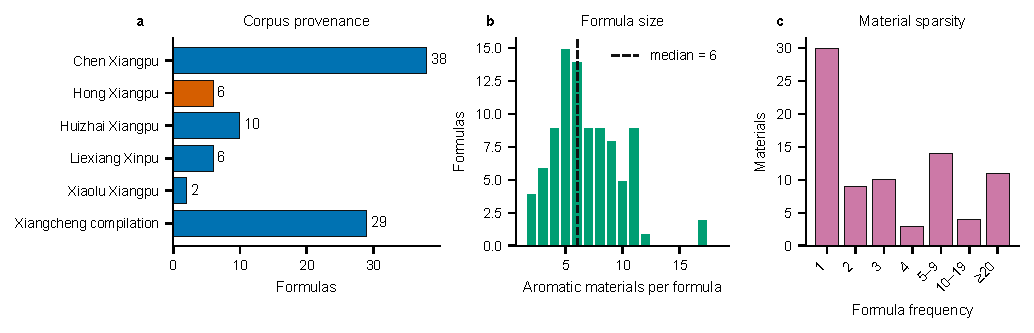
\includegraphics[width=0.98\linewidth]{figures/fig2_corpus.pdf}
\caption{Corpus composition. \textbf{a}, Formula count by historical work group. Vermillion marks the six-formula Hong confirmation work; blue marks the five development and primary work groups. \textbf{b}, Distribution of aromatic material count across all 91 formulas; the dashed line marks the median of six. \textbf{c}, Number of canonical materials by corpus formula frequency. Thirty of 81 materials occur once.}
\label{fig:2}
\end{figure}

\subsection{A directed material graph carries the cross-document gain}

At the registered 50\% observation fraction, the global-frequency baseline reached source-macro hidden-component F1 0.339 and weighted Jaccard 0.379. Weighted Jaccard measures the fraction of total formula mass shared by the reference and prediction. The directed graph reached F1 0.365 and weighted Jaccard 0.388. The locked full decoder reached F1 0.366 and weighted Jaccard 0.387 (Fig. 3; Tables 4 and 5). Its mean work-level F1 difference from frequency was 0.0278. Four of five work groups improved; the source-bootstrap interval was [0.0079, 0.0473], while the exact five-block sign-flip test gave p = 0.125. Five independent work groups produce a coarse exact p-value grid, so the effect magnitude and cross-source pattern are the informative quantities.

The full decoder and graph-only scores were nearly identical. Their mean work-level F1 difference was 0.0010, the source-bootstrap interval was [\ensuremath{-}0.0072, 0.0100], and the exact sign-flip p-value was 0.875. Title similarity and source prevalence therefore did not add stable information after the observed ingredients reached the conditional graph. The graph is the effective model component.

Transfer varied by source. The full decoder reached hidden F1 0.443 on Liexiang Xinpu, 0.396 on Chen Xiangpu, 0.392 on the Xiangcheng compilation, 0.392 on Xiaolu Xiangpu and 0.210 on Huizhai Xiangpu (Fig. 3a; Table 5). Weighted Jaccard ranged from 0.324 to 0.446. Reporting only the pooled mean would conceal this document effect.

After freezing the decoder, we added two competitive set-completion baselines with configurations selected on the five development work splits. Formula k-nearest neighbours reached primary hidden F1 0.343 and PureSVD reached 0.334, compared with 0.365 for the directed graph (Fig. 4a; Table 4). The graph exceeded formula k-nearest neighbours by 0.0223 F1 and PureSVD by 0.0311 at the work level. Formula k-nearest neighbours produced the highest weighted Jaccard, 0.443, because it fixed supplied ratios and interpolated neighbour compositions. Applying the same mass constraint to the full decoder increased weighted Jaccard from 0.387 to 0.427 without changing its selected materials.

Nine formulas had aromatic material-set Jaccard at least 0.8 with a formula from another work group. Removing all nine reduced graph F1 to 0.348 and frequency F1 to 0.322; the graph retained a 0.0259 work-level advantage (Fig. 4b). High-similarity transmission therefore raises absolute performance but does not account for the graph-frequency ordering.

\begin{table}[htbp]
\centering
\small
\caption{Primary source-macro comparison at 50\% observed context. Each metric is averaged first within formula, then within work and finally across works.}
\label{tab:4}
\begin{adjustbox}{max width=\linewidth}
\begin{tabular}{@{}lll@{}}
\toprule
\textbf{Model} & \textbf{Hidden F1 higher is better} & \textbf{Weighted Jaccard higher is better} \\
\midrule
Frequency & 0.339 & 0.379 \\
Formula kNN & 0.343 & 0.443 \\
PureSVD & 0.334 & 0.420 \\
Directed graph & 0.365 & 0.388 \\
Full decoder & 0.366 & 0.387 \\
\bottomrule
\end{tabular}
\end{adjustbox}
\end{table}

\begin{table}[htbp]
\centering
\small
\caption{Work-level hidden-component F1 at 50\% observed context. Work groups, rather than repeated masks, are the independent evaluation blocks.}
\label{tab:5}
\begin{adjustbox}{max width=\linewidth}
\begin{tabular}{@{}lllll@{}}
\toprule
\textbf{Held-out work} & \textbf{Formulas} & \textbf{Frequency F1} & \textbf{Directed graph F1} & \textbf{Full decoder F1} \\
\midrule
Chen Xiangpu & 38 & 0.356 & 0.404 & 0.396 \\
Huizhai Xiangpu & 9 & 0.178 & 0.218 & 0.210 \\
Liexiang Xinpu & 6 & 0.428 & 0.446 & 0.443 \\
Xiaolu Xiangpu & 2 & 0.400 & 0.375 & 0.392 \\
Xiangcheng compilation & 29 & 0.331 & 0.384 & 0.392 \\
\bottomrule
\end{tabular}
\end{adjustbox}
\end{table}

\begin{figure}[htbp]
\centering
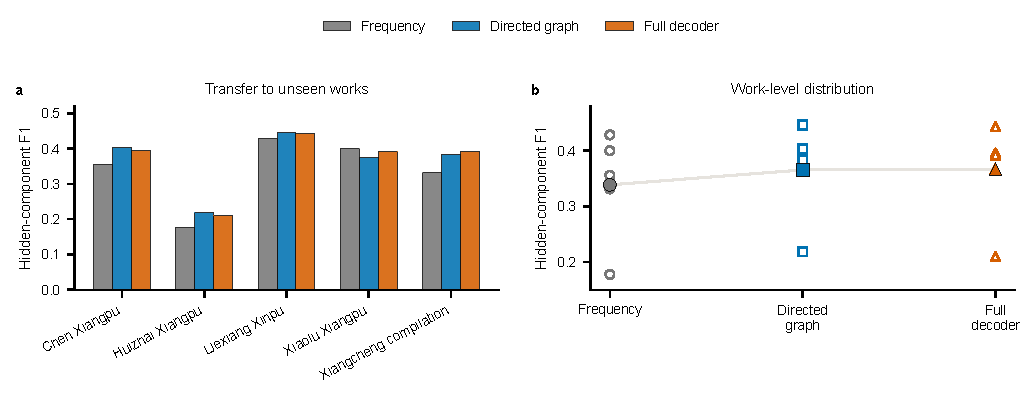
\includegraphics[width=0.98\linewidth]{figures/fig3_primary_performance.pdf}
\caption{Primary source-shifted completion performance. \textbf{a}, Hidden-component F1 by held-out work group for global frequency, directed graph and the locked full decoder at 50\% observed context. Values average all source-pair appearances and five deterministic masks for each formula. \textbf{b}, Work-level values and source-macro means. Open markers show the five work groups; filled markers show their unweighted mean. Work groups form the unit of inference; repeated formula-mask instances do not.}
\label{fig:3}
\end{figure}

\begin{figure}[htbp]
\centering
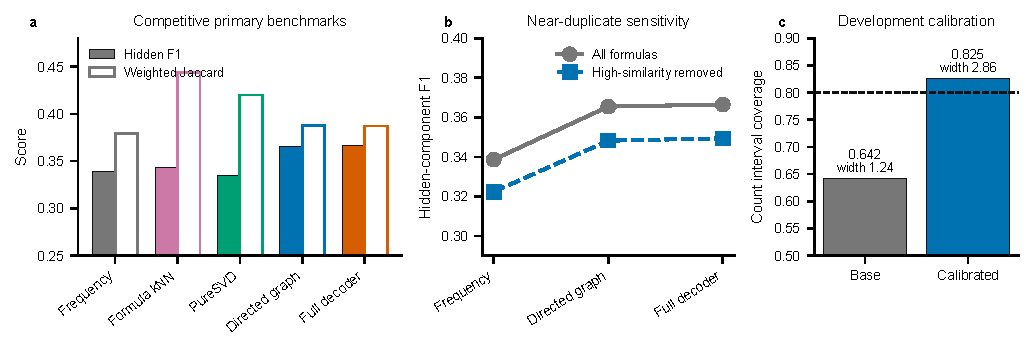
\includegraphics[width=0.98\linewidth]{figures/fig6_stress_tests.pdf}
\caption{Competitive baselines and post-freeze stress tests. \textbf{a}, Source-macro hidden-component F1 and complete-composition weighted Jaccard for frequency, formula k-nearest neighbours, PureSVD, the directed graph and the full decoder. Formula-neighbour and PureSVD configurations were selected on development work splits. \textbf{b}, Hidden-component F1 before and after excluding nine formulas whose material-set Jaccard with another work group was at least 0.8. \textbf{c}, Primary coverage and mean width of the original count interval and the interval expanded by one material using work-held-out development residuals. The dashed line marks nominal 80\% coverage.}
\label{fig:4}
\end{figure}

\subsection{Context amount changes the residual task}

When 25\% of a formula was observed, graph-only reached hidden F1 0.391, compared with 0.381 for frequency and 0.383 for the full decoder. At 50\%, the values were 0.365, 0.339 and 0.366. At 75\%, they were 0.245, 0.232 and 0.244 (Fig. 5a; Table 6). Every value uses the same formula-first, work-second and equal-work macro aggregation as the primary analysis. Hidden F1 falls as the observed fraction rises because the remaining labels form a smaller and harder residual set. At the sparsest 25\% context, graph-only beat the full decoder in all five work groups. The full model's extra channels dilute the strongest signal when little context is available.

Training frequency set a sharp recovery frontier. Hidden-material recall was 0.573 for materials appearing in at least five training formulas, 0.056 for those appearing two to four times, 0.023 for singletons and zero for out-of-vocabulary materials (Fig. 5b). The model most often overpredicted sandalwood, borneol, musk, agarwood and clove. Frequent misses included scrophularia root, spikenard, zhan-grade agarwood, frankincense and clove. Across five deterministic masks, the mean Jaccard similarity between predicted sets was 0.644. The error profile points to data coverage, not decoder depth, as the present performance ceiling.

\begin{table}[htbp]
\centering
\small
\caption{Sensitivity to the observed fraction of each formula. All entries use formula-first, work-second and equal-work aggregation.}
\label{tab:6}
\begin{adjustbox}{max width=\linewidth}
\begin{tabular}{@{}llll@{}}
\toprule
\textbf{Observed fraction} & \textbf{Model} & \textbf{Hidden F1 higher is better} & \textbf{Weighted Jaccard higher is better} \\
\midrule
0.25 & Frequency & 0.381 & 0.265 \\
0.25 & Directed graph & 0.391 & 0.272 \\
0.25 & Full decoder & 0.383 & 0.271 \\
0.5 & Frequency & 0.339 & 0.379 \\
0.5 & Directed graph & 0.365 & 0.388 \\
0.5 & Full decoder & 0.366 & 0.387 \\
0.75 & Frequency & 0.232 & 0.525 \\
0.75 & Directed graph & 0.245 & 0.529 \\
0.75 & Full decoder & 0.244 & 0.525 \\
\bottomrule
\end{tabular}
\end{adjustbox}
\end{table}

\begin{figure}[htbp]
\centering
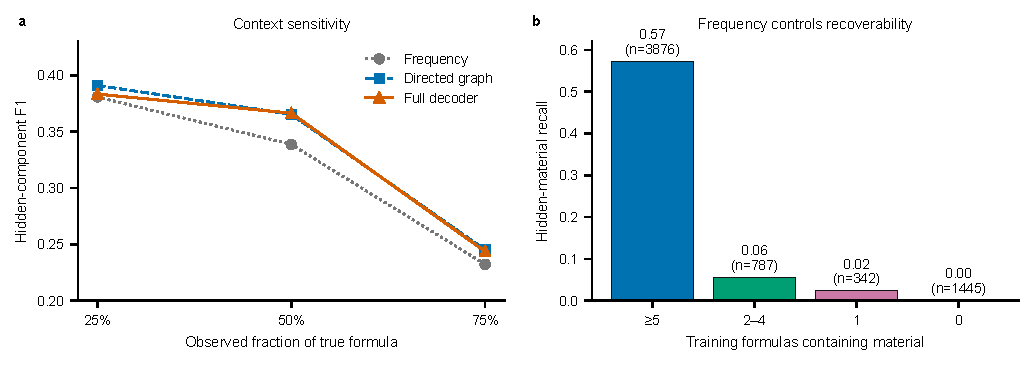
\includegraphics[width=0.98\linewidth]{figures/fig4_robustness.pdf}
\caption{Context and rarity sensitivity. \textbf{a}, Source-macro hidden-component F1 at 25\%, 50\% and 75\% observed formula context. Color, marker and line style redundantly encode the three models. \textbf{b}, Hidden-material recall for the locked decoder grouped by material frequency in the corresponding training folds. Labels report recall and the number of repeated recovery opportunities across source-pair folds and masks.}
\label{fig:5}
\end{figure}

\subsection{Uncertainty outputs are informative but high probabilities remain overconfident}

Across 95,210 hidden candidate decisions, the locked decoder produced a Brier score of 0.0429 and expected calibration error of 0.0236 \cite{ref15}. Those aggregate values are dominated by the large low-probability class. The reliability curve shows close agreement below probability 0.3 and increasing overconfidence above 0.4; the highest bin had mean probability 0.931 and empirical inclusion frequency 0.565 (Fig. 6a; Table 7).

The formula-size posterior underestimated total ingredient count by 0.883 materials on average. Its mean absolute error was 1.190, and the nominal central 80\% interval covered 64.2\% of true counts. Work-held-out development residuals set a one-material expansion without accessing primary labels. The expanded interval covered 82.5\% in primary evaluation, while mean width increased from 1.24 to 2.86 materials (Fig. 4c; Table 7). Conditional on both the selected set and correct material selection, the central 80\% interval from the residual-scaled Dirichlet distribution covered 91.2\% of reference ratios. The selected set contained 63.1\% of all true components. Inclusion probabilities were accurate at low scores, count uncertainty required calibration and ratio intervals were conservative after correct selection.

\begin{table}[htbp]
\centering
\small
\caption{Uncertainty diagnostics for inclusion, ingredient count and composition. Ratio coverage is conditional on correct material selection.}
\label{tab:7}
\begin{adjustbox}{max width=\linewidth}
\begin{tabular}{@{}lll@{}}
\toprule
\textbf{Diagnostic} & \textbf{Estimate} & \textbf{Interpretation} \\
\midrule
Hidden-candidate Brier score & 0.0429 & Lower is better \\
Hidden-candidate ECE & 0.0236 & Ten equal-width bins \\
Base count interval coverage & 0.642 & Nominal level 0.80 \\
Calibrated count interval coverage & 0.825 & Development radius equals one \\
Calibrated count interval mean width & 2.861 & Materials \\
Conditional ratio interval coverage & 0.912 & Conditional on correct selection \\
\bottomrule
\end{tabular}
\end{adjustbox}
\end{table}

\begin{figure}[htbp]
\centering
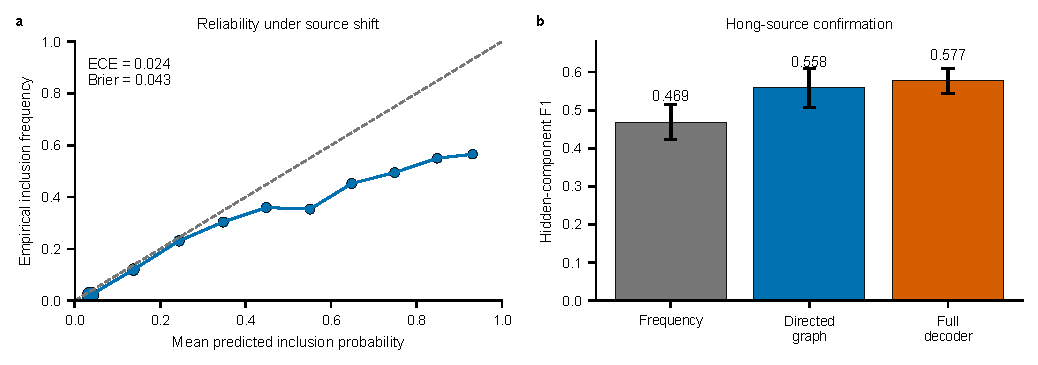
\includegraphics[width=0.98\linewidth]{figures/fig5_uncertainty_confirmation.pdf}
\caption{Probabilistic behavior and confirmation. \textbf{a}, Ten-bin reliability curve for 95,210 hidden candidate decisions from the locked primary decoder. Marker area scales with the square root of bin count; the dashed diagonal marks exact calibration. \textbf{b}, Hidden-component F1 on six Hong-source formulas after model freeze. Bars show the mean across five deterministic masks and error bars show the standard deviation across masks. The confirmation formulas form one historical work group.}
\label{fig:6}
\end{figure}

\subsection{Chemistry tests separate similarity from co-formulation}

Ratio estimation uses compositional-data geometry \cite{ref19}, compounds use radius-2, 2,048-bit Morgan fingerprints \cite{ref20}, and the implementation uses scikit-learn \cite{ref21}. The chemical evidence layer links 18 of 81 materials to 18 specimen-level analytical profiles drawn from 17 publications \cite{ref22,ref23,ref24,ref25,ref26,ref27,ref28,ref29,ref30,ref31,ref32,ref33,ref34,ref35,ref36,ref37,ref38} and 40 PubChem compounds. Each profile retains taxon, plant part, preparation, analytical method and measurement basis. The model also includes physicochemical descriptors and controlled odor tags. A pairwise kernel combines fingerprint Tanimoto similarity, positive physicochemical cosine similarity and positive odor-tag cosine similarity.

The best chemistry-enabled primary-task variant reached development F1 0.3905, compared with 0.3911 for the selected non-chemistry variant. Chemistry was therefore disabled before primary evaluation. The auxiliary odor-to-formula task used 44 legacy formulas and nested leave-one-family-out validation. Odor k-nearest neighbors reached pooled weighted Jaccard 0.2913. The forward-consistent model reached 0.2824, its no-chemistry ablation 0.2835 and shuffled chemistry 0.2863. Pairwise chemical resemblance did not encode historical co-formulation. Similar materials can substitute for one another, while formulas often combine chemically dissimilar materials for contrast, volatility control or processing behavior.

\subsection{Quarantined-source confirmation reproduces the ranking}

After the model and analysis code were frozen, all 85 development formulas were used to predict the six Hong-source formulas. At 50\% observed context, frequency reached hidden F1 0.469, graph-only 0.558 and the full decoder 0.577 (Fig. 6b). Weighted Jaccard values were 0.420, 0.456 and 0.468. The full decoder exceeded frequency by 0.108 F1 across the six formulas. These records share one work group, so they confirm transfer to a new source without adding a sixth independent block to the primary inference.

A fixed case-selection rule chose the seed-17 confirmation formula closest to the six-formula median hidden F1. For \emph{Yinxiang fa}, six of eleven reference materials were observed. The decoder recovered zhan-grade agarwood, borneol and sandalwood; it missed frankincense and licorice and added clove and linglingxiang. Ingredient count was exact, hidden F1 was 0.600 and mass-constrained weighted Jaccard was 0.483 (Table 8). This case shows the intended use of the ranking and its current failure mode: common structural partners are recoverable, while low-frequency components remain difficult.

\begin{table}[htbp]
\centering
\small
\caption{Fixed confirmation case study for Yinxiang fa at seed 17. Blank predicted ratios indicate materials absent from the predicted set.}
\label{tab:8}
\begin{adjustbox}{max width=\linewidth}
\begin{tabular}{@{}lllll@{}}
\toprule
\textbf{Material} & \textbf{Outcome} & \textbf{Reference ratio} & \textbf{Predicted ratio} & \textbf{Inclusion probability} \\
\midrule
agarwood & observed input & 0.066 & 0.066 & 1.000 \\
agarwood zhan grade & recovered hidden & 0.332 & 0.117 & 0.158 \\
borneol family & recovered hidden & 0.013 & 0.099 & 0.617 \\
clove bud & false positive & 0.000 & 0.106 & 0.284 \\
frankincense & missed hidden & 0.066 &  &  \\
licorice & missed hidden & 0.066 &  &  \\
linglingxiang & false positive & 0.000 & 0.120 & 0.440 \\
mao aromatic grass & observed input & 0.266 & 0.266 & 1.000 \\
musk & observed input & 0.053 & 0.053 & 1.000 \\
onycha & observed input & 0.001 & 0.001 & 1.000 \\
patchouli & observed input & 0.001 & 0.001 & 1.000 \\
sandalwood white & recovered hidden & 0.066 & 0.103 & 0.695 \\
spikenard & observed input & 0.066 & 0.066 & 1.000 \\
\bottomrule
\end{tabular}
\end{adjustbox}
\end{table}

\subsection{The complete model runs on ordinary hardware}

Training the locked decoder on all 85 development formulas and 80 materials took a median 0.115 s across 11 serial repetitions on an Apple arm64 system. A prediction with 200 posterior samples took 1.70 ms. The interquartile ranges were 5.28 ms for fitting and 0.14 ms for prediction. The conditional graph uses dense O(NM\ensuremath{{}^{2}}) construction in the reference implementation, although sparse hyperedge accumulation reduces this to O(\ensuremath{\Sigma}\ensuremath{_{i}}|S\ensuremath{_{i}}|\ensuremath{{}^{2}}). With D decoder features and R training masks, logistic fitting uses RNM candidate rows and O(RNMD) work per objective evaluation. The small-data design keeps the full pipeline reproducible on a laptop.

\section{Discussion}

Historical formula completion is tractable when partial ingredients survive and related source traditions provide repeated material structure. The directed graph improved hidden-component F1 over frequency across four of five work groups, exceeded formula-neighbour and low-rank baselines, survived removal of nine high-similarity formulas and reproduced its ordering on the Hong confirmation source. Conditional co-formulation is the transferable signal. Generic text features and the tested chemical kernel added no stable gain.

The model's strongest feature is also its simplest. For every observed material, the graph estimates a smoothed conditional distribution over candidate partners using training formulas only. Averaging these directed conditionals captures asymmetric recipe logic. Musk may strongly predict a common base material even when the reverse conditional is weaker. Bayesian multi-label models have previously exploited label co-occurrence under sparse supervision \cite{ref13}; Xiangji places that principle inside a document-held-out historical benchmark and joins it to explicit formula-size and composition uncertainty models. The source-blocked protocol follows the machine-learning requirement that deployment domains remain outside training data \cite{ref14}. Each historical work defines a domain in this study.

The negative chemistry result sharpens the theory. Molecular odor models \cite{ref4,ref5,ref6,ref7,ref8} and blend predictors \cite{ref9} learn perceptual similarity or descriptor response. Historical ingredient pairing is a complementarity relation. A sandalwood base and a volatile top note may be valuable together because they differ in molecular composition and evaporation behavior. The symmetric kernel collapses substitution and complementarity into one number. A stronger chemistry-aware model should represent directed functional roles and interactions: base versus modifier, volatility ordering, combustion products, odor thresholds and nonlinear mixture suppression. It should train against new formula sources or physical measurements, leaving the present confirmation work untouched.

The task also differs from two adjacent forms of olfactory reconstruction. GC-MS/O can recover odor-active compounds when a physical residue survives \cite{ref3}. Descriptor-to-mixture optimization can design a modern scent that matches a requested profile \cite{ref10}. Xiangji completes a recorded material formula from documentary structure. Its output is a candidate formula completion; sensory identity requires analytical and panel validation. The task is computationally testable because known formulas can be masked and transferred across sources.

\section{Limitations}

The corpus has five primary source blocks, one confirmation block and a long tail of materials supported by one or two formulas. One curator performed the current canonicalization; independent recuration is needed to measure label stability. The model has no combustion or sensory measurements, and the evaluated task assumes that part of the ingredient set is known. A second release should add independently annotated work groups, controlled burn-headspace profiles and ranked expert judgments. Those additions would support full text-to-candidate reconstruction while preserving the current benchmark.

\section{Conclusion}

This study establishes a computational baseline for historical-formulation research. It provides the dataset structure, leakage controls, uncertainty decomposition and negative controls needed to compare stronger models. Across source shift, learned recipe relations carry usable information, while chemical similarity must be modeled as interaction before it can guide historical ingredient pairing.

\section*{Data availability}

The curated formula reference, source locators, source-blocked splits, material ontology, compound-evidence registry, frozen experiment outputs and figure source tables are included in the project repository at \nolinkurl{https://github.com/HongbaiJoe/xiangji-incense-reconstruction-lab} on the \texttt{research/xiangji-cgir-paper} branch. Historical transcriptions remain subject to their recorded source terms; the dataset stores revision URLs and rights metadata for each record.

\section*{Code availability}

Model, evaluation, figure-generation and audit code is available in the same repository and branch. The repository includes a locked environment, deterministic seeds, Make targets and automated tests. An archival DOI will be added before journal submission.

\section*{Acknowledgements}

[Add verified funding and acknowledgements, or state that the work received no specific funding.]

\section*{Author contributions}

[Insert author initials and verified CRediT contributions before submission.]

\section*{Competing interests}

[Insert the authors' verified competing-interest declaration before submission.]

\begin{thebibliography}{99}

\bibitem{ref1}Bembibre, C. \& Strlič, M. Smell of heritage: a framework for the identification, analysis and archival of historic odours. \emph{Herit. Sci.} \textbf{5}, 2 (2017). \nolinkurl{https://doi.org/10.1186/s40494-016-0114-1}

\bibitem{ref2}Lisena, P. \emph{et al.} Capturing the semantics of smell: the Odeuropa data model for olfactory heritage information. In \emph{The Semantic Web} 387-405 (Springer, 2022). \nolinkurl{https://doi.org/10.1007/978-3-031-06981-9_23}

\bibitem{ref3}Paolin, E. \emph{et al.} A systematic approach to the scientific reproduction of historical smells: case study of a 20th-century perfume flask. \emph{npj Herit. Sci.} (2026). \nolinkurl{https://doi.org/10.1038/s40494-026-02699-x}

\bibitem{ref4}Lee, B. K. \emph{et al.} A principal odor map unifies diverse tasks in olfactory perception. \emph{Science} \textbf{381}, 999-1006 (2023). \nolinkurl{https://doi.org/10.1126/science.ade4401}

\bibitem{ref5}Gutiérrez, E. D., Dhurandhar, A., Keller, A., Meyer, P. \& Cecchi, G. A. Predicting natural language descriptions of mono-molecular odorants. \emph{Nat. Commun.} \textbf{9}, 4979 (2018). \nolinkurl{https://doi.org/10.1038/s41467-018-07439-9}

\bibitem{ref6}Keller, A. \emph{et al.} Predicting human olfactory perception from chemical features of odor molecules. \emph{Science} \textbf{355}, 820-826 (2017). \nolinkurl{https://doi.org/10.1126/science.aal2014}

\bibitem{ref7}Debnath, T., Prasetyawan, D. \& Nakamoto, T. Predicting odor perception of mixed scent from mass spectrometry. \emph{J. Electrochem. Soc.} \textbf{168}, 117505 (2021). \nolinkurl{https://doi.org/10.1149/1945-7111/ac33e0}

\bibitem{ref8}Hamel, E. A. \emph{et al.} Pyrfume: a window to the world's olfactory data. \emph{Sci. Data} \textbf{11}, 1220 (2024). \nolinkurl{https://doi.org/10.1038/s41597-024-04051-z}

\bibitem{ref9}Sisson, L., Barsainyan, A. A., Sharma, M. \& Kumar, R. Deep learning for odor prediction on aroma-chemical blends. \emph{ACS Omega} \textbf{10}, 8980-8992 (2025). \nolinkurl{https://doi.org/10.1021/acsomega.4c07078}

\bibitem{ref10}Aleixandre, M., Prasetyawan, D. \& Nakamoto, T. Automatic scent creation by cheminformatics method. \emph{Sci. Rep.} \textbf{14}, 31284 (2024). \nolinkurl{https://doi.org/10.1038/s41598-024-82654-7}

\bibitem{ref11}Sorbi, M., Moccozet, L. \& Marchand-Maillet, S. Weakly supervised named entity recognition for historical texts. In \emph{Proceedings of the 10th Joint SIGHUM Workshop} 48-65 (ACL, 2026). \nolinkurl{https://doi.org/10.18653/v1/2026.latechclfl-1.6}

\bibitem{ref12}Goel, M. \emph{et al.} Deep learning based named entity recognition models for recipes. In \emph{Proceedings of LREC-COLING 2024} 4542-4554 (ELRA and ICCL, 2024).

\bibitem{ref13}Zhao, H., Rai, P., Du, L. \& Buntine, W. Bayesian multi-label learning with sparse features and labels, and label co-occurrences. \emph{Proc. Mach. Learn. Res.} \textbf{84}, 1943-1951 (2018).

\bibitem{ref14}Koh, P. W. \emph{et al.} WILDS: a benchmark of in-the-wild distribution shifts. \emph{Proc. Mach. Learn. Res.} \textbf{139}, 5637-5664 (2021).

\bibitem{ref15}Guo, C., Pleiss, G., Sun, Y. \& Weinberger, K. Q. On calibration of modern neural networks. \emph{Proc. Mach. Learn. Res.} \textbf{70}, 1321-1330 (2017).

\bibitem{ref16}Cover, T. M. \& Hart, P. E. Nearest neighbor pattern classification. \emph{IEEE Trans. Inf. Theory} \textbf{13}, 21-27 (1967). \nolinkurl{https://doi.org/10.1109/TIT.1967.1053964}

\bibitem{ref17}Cremonesi, P., Koren, Y. \& Turrin, R. Performance of recommender algorithms on top-N recommendation tasks. In \emph{Proceedings of the Fourth ACM Conference on Recommender Systems} 39-46 (ACM, 2010). \nolinkurl{https://doi.org/10.1145/1864708.1864721}

\bibitem{ref18}Angelopoulos, A. N. \& Bates, S. Conformal prediction: a gentle introduction. \emph{Found. Trends Mach. Learn.} \textbf{16}, 494-591 (2023). \nolinkurl{https://doi.org/10.1561/2200000101}

\bibitem{ref19}Aitchison, J. The statistical analysis of compositional data. \emph{J. R. Stat. Soc. B} \textbf{44}, 139-160 (1982). \nolinkurl{https://doi.org/10.1111/j.2517-6161.1982.tb01195.x}

\bibitem{ref20}Rogers, D. \& Hahn, M. Extended-connectivity fingerprints. \emph{J. Chem. Inf. Model.} \textbf{50}, 742-754 (2010). \nolinkurl{https://doi.org/10.1021/ci100050t}

\bibitem{ref21}Pedregosa, F. \emph{et al.} Scikit-learn: machine learning in Python. \emph{J. Mach. Learn. Res.} \textbf{12}, 2825-2830 (2011).

\bibitem{ref22}Ngan, T. T. K. \emph{et al.} Chemical components of agarwood (\emph{Aquilaria crassna}) essential oils grown in various regions of Asia. \emph{Asian J. Chem.} \textbf{32}, 36-40 (2020). \nolinkurl{https://doi.org/10.14233/ajchem.2020.22177}

\bibitem{ref23}Fatima, T. \emph{et al.} Assessment of morphological and genetic variability through genic microsatellite markers for essential oil in sandalwood (\emph{Santalum album} L.). \emph{3 Biotech} \textbf{9}, 252 (2019). \nolinkurl{https://doi.org/10.1007/s13205-019-1758-9}

\bibitem{ref24}Di Stefano, V., Schillaci, D., Cusimano, M. G., Rishan, M. \& Rashan, L. In vitro antimicrobial activity of frankincense oils from \emph{Boswellia sacra} grown in different locations of the Dhofar region. \emph{Antibiotics} \textbf{9}, 195 (2020). \nolinkurl{https://doi.org/10.3390/antibiotics9040195}

\bibitem{ref25}Ben Hassine, D. \emph{et al.} Clove buds essential oil: the impact of grinding on the chemical composition and its biological activities involved in consumer health security. \emph{BioMed Res. Int.} \textbf{2021}, 9940591 (2021). \nolinkurl{https://doi.org/10.1155/2021/9940591}

\bibitem{ref26}Firmino, D. F. \emph{et al.} Antibacterial and antibiofilm activities of \emph{Cinnamomum} sp. essential oil and cinnamaldehyde. \emph{Sci. World J.} \textbf{2018}, 7405736 (2018). \nolinkurl{https://doi.org/10.1155/2018/7405736}

\bibitem{ref27}Hu, Q.-P., Cao, X.-M., Hao, D.-L. \& Zhang, L.-L. Chemical composition and biological activities of \emph{Cyperus rotundus} rhizome essential oil. \emph{Sci. Rep.} \textbf{7}, 45231 (2017). \nolinkurl{https://doi.org/10.1038/srep45231}

\bibitem{ref28}Han, X., Beaumont, C. \& Stevens, N. Chemical composition analysis and in vitro biological activities of ten essential oils in human skin cells. \emph{Biochim. Open} \textbf{5}, 1-7 (2017). \nolinkurl{https://doi.org/10.1016/j.biopen.2017.04.001}

\bibitem{ref29}Hu, D. \emph{et al.} Comparison and identification of the aroma-active compounds in the root of \emph{Angelica dahurica}. \emph{Molecules} \textbf{24}, 4352 (2019). \nolinkurl{https://doi.org/10.3390/molecules24234352}

\bibitem{ref30}Andola, H. C., Lohani, H., Chauhan, N., Gwari, G. \& Bhandari, U. Volatile constituents of \emph{Saussurea costus} roots cultivated in the Uttarakhand Himalayas. \emph{Pharmacogn. Res.} \textbf{5}, 179 (2013). \nolinkurl{https://doi.org/10.4103/0974-8490.112424}

\bibitem{ref31}Zou, L. \emph{et al.} Comparison of chemical profiles between synthetic borneol and natural borneol. \emph{Molecules} \textbf{22}, 1446 (2017). \nolinkurl{https://doi.org/10.3390/molecules22091446}

\bibitem{ref32}Li, D. \emph{et al.} The musk chemical composition and microbiota of Chinese forest musk deer males. \emph{Sci. Rep.} \textbf{6}, 18975 (2016). \nolinkurl{https://doi.org/10.1038/srep18975}

\bibitem{ref33}Xue, G. Q. \emph{et al.} Chemical constituents of \emph{Scrophularia ningpoensis} root. \emph{Zhong Yao Cai} \textbf{37}, 1597-1599 (2014). \nolinkurl{https://pubmed.ncbi.nlm.nih.gov/25857160/}

\bibitem{ref34}Farag, M. A. \& Wessjohann, L. A. Volatiles profiling in medicinal licorice roots using steam distillation and solid-phase microextraction coupled to chemometrics. \emph{J. Food Sci.} \textbf{77} (2012). \nolinkurl{https://doi.org/10.1111/j.1750-3841.2012.02927.x}

\bibitem{ref35}Fernandez, X. \emph{et al.} Chemical composition of the essential oils from Turkish and Honduras \emph{Styrax}. \emph{Flavour Fragr. J.} \textbf{20}, 70-73 (2005). \nolinkurl{https://doi.org/10.1002/ffj.1370}

\bibitem{ref36}Raza, M. H. \emph{et al.} Comparative study of \emph{Foeniculum vulgare} seed oils obtained by three distillation methods. \emph{Food Sci. Nutr.} \textbf{12}, 10535-10549 (2024). \nolinkurl{https://doi.org/10.1002/fsn3.4593}

\bibitem{ref37}Guo, S. \emph{et al.} The chemical composition of essential oils from \emph{Cinnamomum camphora}. \emph{Int. J. Mol. Sci.} \textbf{17}, 1836 (2016). \nolinkurl{https://doi.org/10.3390/ijms17111836}

\bibitem{ref38}Miyazawa, M., Minamino, Y. \& Kameoka, H. Volatile components of the rhizomes of \emph{Rheum palmatum} L. \emph{Flavour Fragr. J.} \textbf{11}, 57-60 (1996). \nolinkurl{https://doi.org/10.1002/(SICI})1099-1026(199601)11:1\%3C57::AID-FFJ549\%3E3.0.CO;2-K

\end{thebibliography}

\clearpage

\end{document}
